\documentclass[a4paper]{article} 
\usepackage[UTF8]{ctex}
\usepackage{tikz}
\usetikzlibrary{intersections}
\usetikzlibrary{angles}
\usetikzlibrary{quotes}

\tikzset{leader/.style = {thin,gray}}
\tikzset{border/.style ={very thick,color=#1},border/.default=blue}

\newcommand{\gradei}[1]{{\fontspec{SJQY} A}{#1}}
\newcommand{\gradeii}[1]{{\fontspec{SJQY} B}{#1}}
\newcommand{\gradeiii}[1]{{\fontspec{SJQY} C}{#1}}
\newcommand{\steeliii}[2]{{#1}\gradeiii{#2}}
\newcommand{\steelii}[2]{{#1}\gradeii{#2}}
\newcommand{\steeli}[2]{{#1}\gradei{#2}}

\begin{document}
% We are working on
% \begin{tikzpicture}
% \draw (-1.5,0) -- (1.5,0);
% \draw (0,-1.5) -- (0,1.5);
% \end{tikzpicture}

% 最基本的元素是:路径(path)。

% 一个参数的形式:
% \tikz{\draw (0,0) --(1.5,0)}

% \tikz \draw (0,0) -- (1.0,0) -- (1.0,1.0) -- (0,1.0) -- (0,0); 

% \tikz \draw (0,0) .. controls(0.5,0.5) and (1.5,0.5) .. (2,0); 

% \tikz \draw (-1.5,0) -- (1.5,0) -- (0,-1.5) -- (0,1.5);

% \begin{tikzpicture}
% \draw (-1.5,0) -- (1.5,0);
% \draw (0,-1.5) -- (0,1.5);
% \draw (-1,0) .. controls (-1,0.555) and (-0.555,1) .. (0,1)
% .. controls (0.555,1) and (1,0.555) .. (1,0);
% \end{tikzpicture}

% \tikz \draw (0,0) circle [radius=10pt];

% \tikz \filldraw[gray] (0,0) circle [radius=2pt];

% \tikz \draw (0,0) rectangle (0.5,0.5);

% \tikz \draw[step=.5cm,gray,very thin] (-1.4,-1.4) grid (1.4,1.4);

% \tikzset{help lines/.style={color=blue!50,very thin}}
% \tikz \draw[help lines] (0,0) -- (10,0);

% 自定义风格,带参数:
% \begin{tikzpicture}
% [Karl’s grid/.style ={help lines,color=#1!50},
% Karl’s grid/.default=blue]
% \draw[Karl’s grid] (0,0) grid (1.5,2);
% \draw[Karl’s grid=red] (2,0) grid (3.5,2);
% \end{tikzpicture}

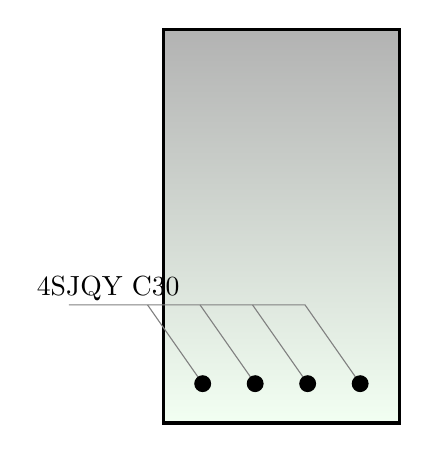
\begin{tikzpicture}
 

\shadedraw[border=black,top color=gray!60!white,bottom color=green!5!white] (0,0) rectangle (3,5);

\draw[leader] (0.5,0.5) -- +(-0.7,1.0);
\draw[leader] (1.16667,0.5) -- +(-0.7,1.0);
\draw[leader] (1.8333,0.5) -- +(-0.7,1.0);
\draw[leader] (2.5,0.5) -- ++(-0.7,1.0) -- ++(-3.0,0);

\draw (-.7cm,1.7cm) node {\steeliii{4}{30}};
\filldraw (0.5,0.5) circle [radius=0.1];
\filldraw (1.16667,0.5) circle [radius=0.1];
\filldraw (1.8333,0.5) circle [radius=0.1];
\filldraw (2.5,0.5) circle [radius=0.1];

\end{tikzpicture}

\tikz \draw (0,0) rectangle (1,1) (0,0) parabola (1,1);
\tikz \shade[ball color=green] (9,.5) circle (.5cm);
\tikz \shade[ball color=green] (12,.5) circle (.2cm);

\tikz \draw[color=blue,dashed ] (0,0) -- (1,0) -- +(0cm,1cm) --cycle; 

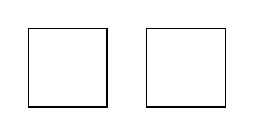
\begin{tikzpicture}
\def\rectanglepath{-- ++(1cm,0cm) -- ++(0cm,1cm)-- ++(-1cm,0cm) -- cycle}
\draw (0,0) \rectanglepath;
\draw (1.5,0) \rectanglepath;
\end{tikzpicture}


\begin{tikzpicture}
\path [name path=upward line] (1,0) -- (1,1);
\path [name path=sloped line] (0,0) -- (30:1.5cm); % a bit longer, so that there is an intersection
\draw [name intersections={of=upward line and sloped line, by=x}]
[very thick,orange] (1,0) -- (x) -- (0,0) -- cycle;
\end{tikzpicture}

\tikz \draw (0,0) -- (0,0.5) [xshift=2pt] (0,0) -- (0,0.5);
\tikz \foreach \x in {0,1,2} \draw (0,\x) rectangle +(0.2,0.2);

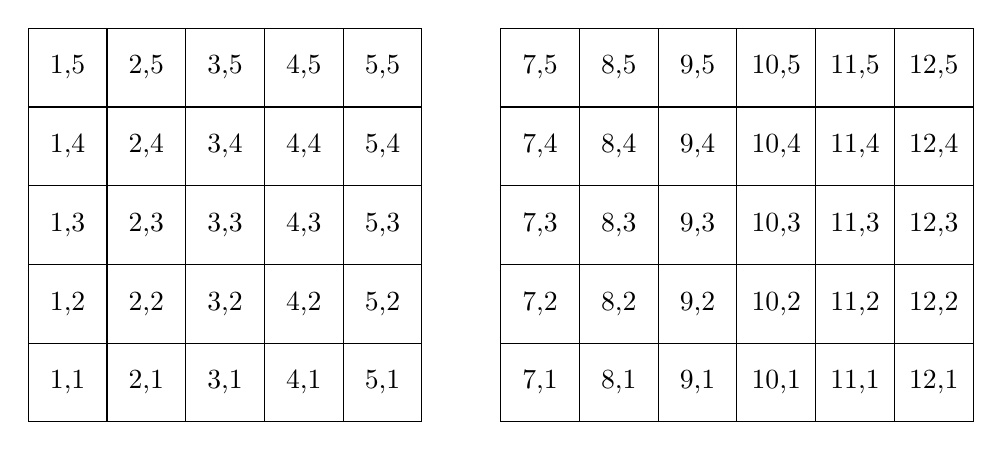
\begin{tikzpicture}
\foreach \x in {1,2,...,5,7,8,...,12}
   \foreach \y in {1,...,5}
   {
     \draw (\x,\y) +(-.5,-.5) rectangle ++(.5,.5);
     \draw (\x,\y) node{\x,\y};
   }
\end{tikzpicture}
  
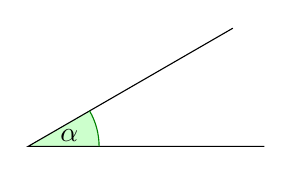
\begin{tikzpicture}[scale=3]
  \coordinate (A) at (1,0);
  \coordinate (B) at (0,0);
  \coordinate (C) at (30:1cm);

  \draw (A) -- (B) -- (C)
      pic[draw=green!50!black, fill=green!20, angle radius=9mm,
         "$\alpha$"] {angle = A--B--C};
\end{tikzpicture}

\end{document}

%%% Local Variables:
%%% mode: latex
%%% TeX-master: t
%%% End:
